\documentclass[11pt, twocolumn]{article}  
% Paquetes básicos para incluir gráficos, matemáticas y fuentes
\usepackage{graphicx}   % Para incluir gráficos
\usepackage{amsmath}    % Para mejorar la presentación de fórmulas matemáticas
\usepackage{amssymb}    % Símbolos matemáticos adicionales
\usepackage{amsfonts}   % Fuentes adicionales para matemáticas
\usepackage[utf8]{inputenc} % Codificación UTF-8 para acentos y caracteres especiales
\usepackage[spanish]{babel} % Configura el idioma en español para ajustar rótulos automáticamente

% Configuración de página y márgenes
\usepackage{geometry} % Control de márgenes y tamaño de página
\geometry{letterpaper, margin=0.75in} % Define el tamaño del papel y establece márgenes

% Configuración de fuente y estilo de texto
\usepackage{times} % Usa la fuente Times para todo el documento

% Paquete para leyendas y figuras
\usepackage{caption} % Controla el formato de las leyendas en figuras y tablas
\captionsetup{font=small, labelfont=bf} % Reduce el tamaño de las leyendas y pone en negrita los rótulos

% Paquetes adicionales para formato y control del documento
\usepackage{abstract}   % Proporciona un formato de resumen adecuado para artículos científicos
\usepackage{float}      % Controla la ubicación de las figuras
\usepackage{placeins}   % Permite controlar la posición de los elementos flotantes, como figuras y tablas
\usepackage{titlesec}   % Personalización de títulos de secciones

% Configuración del formato de títulos y subtítulos
\titleformat{\section}{\large\bfseries}{\thesection}{1em}{} % Estilo de secciones principales
\titleformat{\subsection}{\normalsize\bfseries}{\thesubsection}{1em}{} % Estilo de subsecciones
\titleformat{\subsubsection}{\normalsize\itshape}{\thesubsubsection}{1em}{} % Estilo de subsubsecciones

% Título, autores y fecha
\title{\vspace{-1cm}Optimización del Arbitraje de BESS mediante el Pronóstico del Costo Marginal de Generación en el Sistema Eléctrico Nacional Chileno}
\author{
    \begin{tabular}[t]{c} % Para alinear los autores en una tabla
        Gonzalo Iglesias, Nicolás Sotelo, Maximiliano Cruz \\
        Pontificia Universidad Católica de Chile \\
    \end{tabular}
}
\date{3 de noviembre de 2024} % Especifica la fecha de publicación

\begin{document}

% Inicio de contenido en dos columnas
\twocolumn[
\maketitle % Genera el título y autores

% Espacio reducido entre título y resumen
\vspace{-1.5em}  
\begin{onecolabstract}
\noindent % Elimina sangría en la primera línea
\small % Reduce el tamaño de fuente del resumen
El precio de venta de la energía (Costo Marginal o CMg) en el mercado spot chileno se determina por el costo de la unidad más cara despachada en el sub-sistema respectivo. Para optimizar la rentabilidad de BESS que retiran e inyectan al sistema mediante el mercado spot es crucial tener una estimación de los costos en el corto plazo (24-48 horas). Este trabajo realiza un análisis de rendimiento de tres arquitecturas avanzadas de deep learning para el pronóstico del CMg: una Red Neuronal Convolucional de Grafos (GCN) combinada con GRU, un Transformer para series temporales (Informer) y un modelo híbrido Transformer + CNN (TFT) para capturar patrones estacionales y relaciones de largo alcance. El proyecto busca identificar la arquitectura más precisa para apoyar la toma de decisiones en el almacenamiento energético, optimizando el arbitraje.
\end{onecolabstract}
\vspace{0.5cm} % Espacio debajo del abstract para separar del contenido
]

% Inicio de la primera sección
\section{Introducción}
\vspace{-1em} % Reduce espacio innecesario tras el título de la sección
Durante la última década, Chile ha experimentado un rápido crecimiento en la penetración de energías renovables no convencionales (ERNC) en la zona norte, lo que no ha sido acompañado por un aumento equivalente en la capacidad de transmisión. Esto ha causado congestiones en la transmisión, lo cual afecta el Costo Marginal de Generación (CMg) al generar precios bajos o nulos en las zonas con sobreoferta.

Este proyecto presenta una adaptación de arquitecturas avanzadas de deep learning al contexto del sistema eléctrico chileno, caracterizado por una alta penetración de ERNC y congestionamiento en la transmisión, factores que impactan la variabilidad en el CMg. A diferencia de estudios previos, nuestra propuesta se enfoca en capturar tanto las relaciones espaciales entre zonas de transmisión como los patrones temporales de largo alcance, empleando un enfoque multimodal.

% Figura 1: Cambio en la matriz de generación
\begin{figure}[!b]
    \centering
    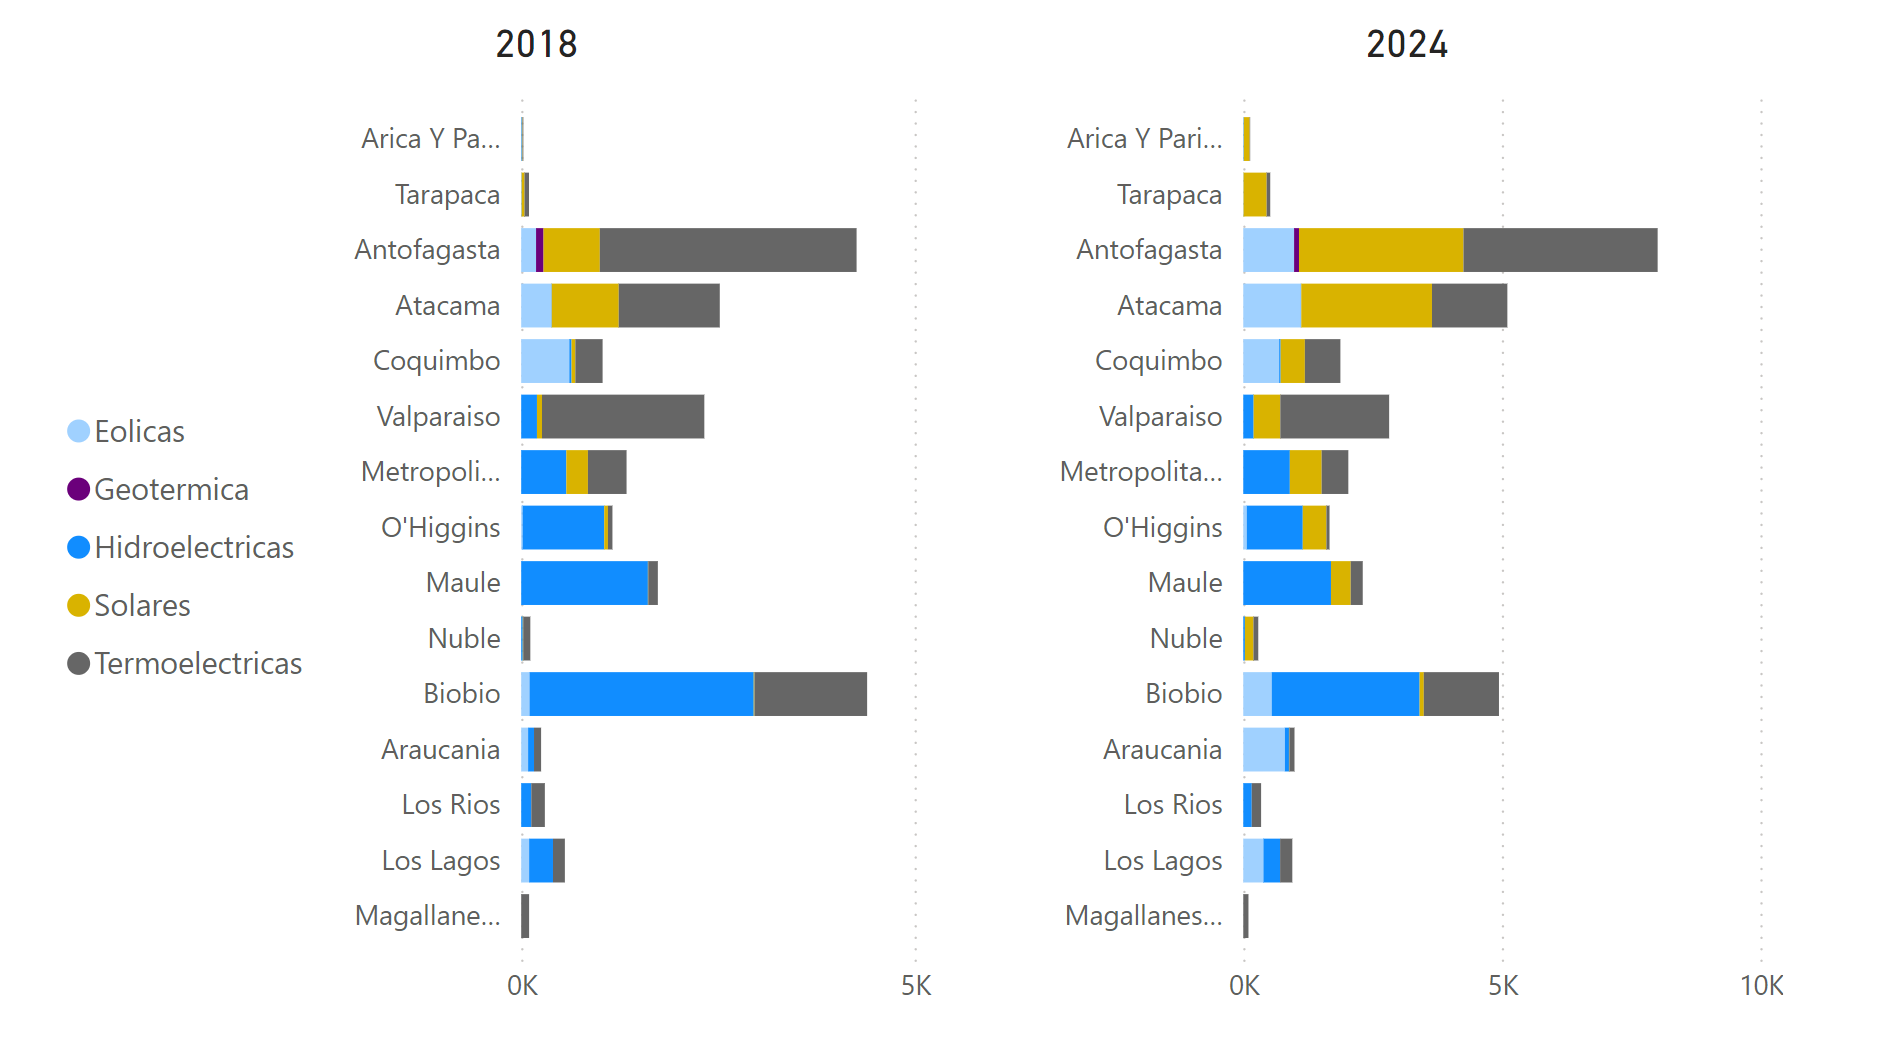
\includegraphics[width=0.85\columnwidth]{img_entrega_1/matriz_sist.png}
    \caption{Cambio en la Matriz de Generación del SEN}
    \label{fig:matriz_sistema}
\end{figure}

Para maximizar la rentabilidad de BESS, es crucial identificar patrones en la variabilidad del CMg en el corto plazo (24-48 horas). En este proyecto se evaluarán tres arquitecturas de deep learning con el objetivo de comparar su efectividad en la predicción de CMg y contribuir al conocimiento científico mediante el análisis de su capacidad para capturar patrones de largo y corto alcance en series temporales energéticas.

% Figura 2: Comparación de perfil CMg
\begin{figure}[!b]
    \centering
    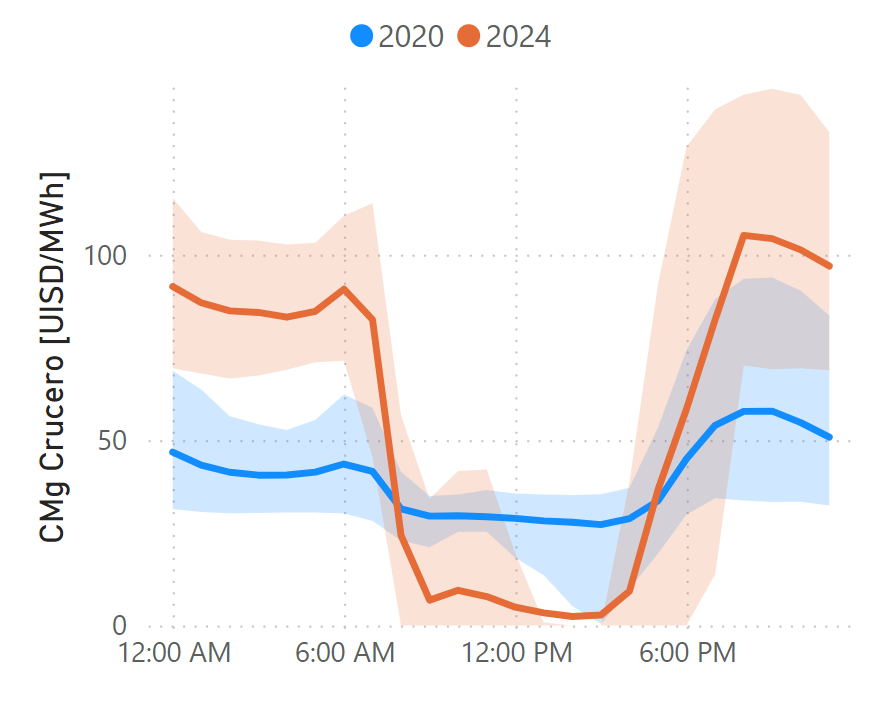
\includegraphics[width=0.85\columnwidth]{img_entrega_1/cmg_comparacion.png}
    \caption{Comparación perfil diario CMg promedio pre y post escenario de congestión en barra Crucero 220kV}
    \label{fig:cmg_comparacion}
\end{figure}

% Metodología
\section{Metodología}
\subsection{Datos}
Para el entrenamiento de los modelos, contamos con una serie de datos que son considerados drivers claves del costo marginal, adicionales al CMg histórico, el cual será nuestra variable objetivo. Los datos incluyen:

\begin{itemize}
    \item \textbf{Demanda Nacional}: demanda eléctrica en MW, desde 2018 con resolución horaria.
    \item \textbf{Disponibilidad de ERNC}: pronóstico de ERNC en MW por central, por hora.
    \item \textbf{Matriz de Generación}: potencia instalada por tecnología en MW desde 2018.
    \item \textbf{Cotas de Embalse}: niveles de embalse de las principales centrales hidroeléctricas.
\end{itemize}

Estos datos forman una serie temporal extensa con variaciones estacionales y eventos de congestión, lo cual presenta un desafío en el modelado debido a la alta dimensionalidad y variabilidad intrínseca.

% Descripción de Modelos
\subsection{Modelos}
Para abordar el problema, evaluamos tres arquitecturas de deep learning:

\begin{enumerate}
    \item \textbf{GCN + GRU}: combina una GCN para modelar la red de transmisión, capturando interacciones espaciales entre distintas zonas, con una capa GRU para manejar dependencias temporales en la serie.
    \item \textbf{Informer}: un Transformer optimizado para series largas, ideal para detectar patrones de largo alcance en la demanda y disponibilidad energética, aprovechando su arquitectura para el procesamiento eficiente de secuencias.
    \item \textbf{TFT (Transformer + CNN)}: utiliza CNN para captar estacionalidades de corto plazo y mecanismos de atención para identificar relaciones de largo plazo, lo que resulta útil en contextos de variabilidad del CMg.
\end{enumerate}

La elección de estos modelos responde a su capacidad para capturar tanto relaciones espaciales (a través de GCN) como dependencias de largo alcance (mediante el Transformer). Esto permite adaptar las predicciones de CMg al contexto único del sistema energético chileno.

% Conclusión
\section{Conclusión}
Este proyecto proporciona un enfoque comparativo para la predicción del CMg en el sistema energético chileno, utilizando arquitecturas avanzadas de deep learning. A través del análisis del rendimiento de GCN + GRU, Informer y TFT, esperamos identificar la arquitectura que mejor capte la complejidad espaciotemporal del CMg, optimizando el arbitraje en BESS y aportando un nuevo enfoque para el manejo de la volatilidad en sistemas energéticos.

\end{document}
